%%%%%%%%%%%%%%%%%%%%%%%%%%%%%%%%%%%%%%%%%%%%%%%%%%%%%%%%%%%%%%%%%%%%%%%%%%%%%%%%
%2345678901234567890123456789012345678901234567890123456789012345678901234567890
%        1         2         3         4         5         6         7         8

\documentclass[letterpaper, 10 pt, conference]{ieeeconf}  % Comment this line out
                                                          % if you need a4paper
%\documentclass[a4paper, 10pt, conference]{ieeeconf}      % Use this line for a4
                                                          % paper

\IEEEoverridecommandlockouts                              % This command is only
                                                          % needed if you want to
                                                          % use the \thanks command
\overrideIEEEmargins
% See the \addtolength command later in the file to balance the column lengths
% on the last page of the document



% The following packages can be found on http:\\www.ctan.org
%\usepackage{graphics} % for pdf, bitmapped graphics files
%\usepackage{epsfig} % for postscript graphics files
%\usepackage{mathptmx} % assumes new font selection scheme installed
%\usepackage{times} % assumes new font selection scheme installed
\usepackage{amsmath} % assumes amsmath package installed
\usepackage{amssymb}  % assumes amsmath package installed
\usepackage{boldline}
\usepackage{array,multirow}
\usepackage{hyperref}
\usepackage{color}
\usepackage{graphicx}
\graphicspath{ {images/} }
\definecolor{light-gray}{gray}{0.95}
\newcommand{\code}[1]{\colorbox{light-gray}{\texttt{#1}}}
\DeclareMathOperator*{\argmax}{arg\,max}
\usepackage{bbm}


\title{\LARGE \bf
Preparation of Papers for IEEE Sponsored Conferences \& Symposia*
}

\author{ \parbox{3 in}{\centering Tamir Bennatan
         {\tt\small tamir.bennatan@mail.mcgill.ca}}
         \hspace*{ 0.5 in}
         \parbox{3 in}{ \centering Pradeep Misra**
         {\tt\small pmisra@cs.wright.edu}}
}


\begin{document}



\maketitle
\thispagestyle{empty}
\pagestyle{empty}


%%%%%%%%%%%%%%%%%%%%%%%%%%%%%%%%%%%%%%%%%%%%%%%%%%%%%%%%%%%%%%%%%%%%%%%%%%%%%%%%
\begin{abstract}

This is a bunch of filler. It is here so that I don't screw myself over while formatting.This is a bunch of filler. It is here so that I don't screw myself over while formatting.This is a bunch of filler. It is here so that I don't screw myself over while formatting.This is a bunch of filler. It is here so that I don't screw myself over while formatting.This is a bunch of filler. It is here so that I don't screw myself over while formatting.This is a bunch of filler. It is here so that I don't screw myself over while formatting.This is a bunch of filler. It is here so that I don't screw myself over while formatting.This is a bunch of filler. It is here so that I don't screw myself over while formatting.This is a bunch of filler. It is here so that I don't screw myself over while formatting.This is a bunch of filler. It is here so that I don't screw myself over while formatting.This is a bunch of filler. It is here so that I don't screw myself over while formatting.This is a bunch of filler. It is here so that I don't screw myself over while formatting.This is a bunch of filler. It is here so that I don't screw myself over while formatting.This is a bunch of filler. It is here so that I don't screw myself over while formatting.

\end{abstract}


%%%%%%%%%%%%%%%%%%%%%%%%%%%%%%%%%%%%%%%%%%%%%%%%%%%%%%%%%%%%%%%%%%%%%%%%%%%%%%%%
\section{INTRODUCTION}

In January of 2017, Quora – a popular question and answer website, released a dataset consisting of pairs of questions from their site, and labels indicating if the questions have the same intent. Shortly thereafter, they used this dataset to start a Kaggle competition, offering \$25,000 to the competitors who build the best models for predicting whether a pair of questions are duplicates, in terms of log-loss error. 

The ability to identify duplicate questions is important for question-answer sites like Quora; duplicate questions make it harder to find the best answer for a particular question, and limit the outreach of each individual answer contributed to the site.

Key to the problem of duplicate question detection is the ability to model semantic similarities between pairs of text. This is an important component of many Natural Language Processing (NLP) applications, including information retrieval (Jurafsky \& Martin; 2009), automatic summarization (Lin \& Hovy; 2003) and text classification (Li \& Roth; 2002). 

In this paper, we describe three feature sets designed to capture  the semantic relationship between questions. We then evaluate the relative importance of these features for the duplicate question detection task. Each of these feature sets are inspired by different intuitions about what characterizes semantic similarity, and are engineered using techniques used in wide ranging NLP tasks. 

The first feature set is based on Term Frequency-Inverse Document Frequency (Tf-Idf) scores. Tf-Idf scores have been shown to be an effective way to model the relative importance of words within a document (Rajaraman \& Ullman; 2011). As such, we propose a set of features which measure the similarity of two questions based on the similarity of the important words in each question.

The second feature set attempts to distinguish between questions based on broad categorizations of their expected answer type - a process called question classification. Using a dataset of 5500 factoid questions, annotated with their answer type (Lin \& Roth; 2002), we fit a series of deep neural network models that predict the answer type of a question. We then used the predictions of these models on the Quora dataset as features for the question deduplication task.

The final feature set uses a framework for creating knowledge-based  semantic similarity scores between sentences (Mihalcea et al; 2006). These scores are calculated using semantic similarity metrics of the words in each sentence, where these metrics are defined in relation to a semantic network, such as WordNet (Miller; 1995). We implement and test the utility of these scores, as well as extend this framework by incorporating neural word embeddings.

We first trained a baseline classifier on standard syntactic and neural features. We then augmented these baseline features with different subsets of the features mentioned above, and re-trained our classifiers with these new features. In this paper, we discuss the usefulness of our proposed feature sets in the duplicate question detection task.


\section{RELATED WORK}

To achieve high accuracy, many competitors in the Kaggle competition incorporated hundreds of features and stacked many classifiers when making predictions. Most successful competitors incorporated Long Short Term Memory Recurrent Neural Networks (LSTM) in their submissions. Two LSTM variants proved especially useful: Siamese LSTMs and LSTMs with neural attention.

Siamese LSTMs are composed of two or more LSTM layers which have tied weights. When trained on paired examples, siamese LSTMs have been shown to be effective in semantic similarity and entailment tasks, for they construct sophisticated representations of semantic relationships between input examples (Mueller et al; 2016). This property is applicable to detecting question deduplication, since at its core the duplicate question detection task is one one of detecting semantic coincidence between pairs of input sentences.

Neural attention, when coupled with LSTMs, is a mechanism which allows a LSTM to pay selective attention to the outputs of intermediate LSTM units. This technique has proven to improve the performance of LSTMs in various Natural Language Inference tasks (Rocktäschel et al.; 2016).

Our work differs from that of the top competitors in that our main objective was not to maximize the performance of our models, but rather to craft novel linguistic features and evaluate their predictiveness. Thus, we did not focus on building sophisticated deep learning models, for it is typically difficult to determine the relative importance of different text features using a deep learning model. Instead, we drew inspiration from techniques used in other NLP tasks build features that capture our intuition about what it means for two texts to be semantically similar.


\section{QUORA DATA SET}

The dataset released by Quora consists of 404290 pairs of questions posted to the site. 36.9\% of pairs are labeled as duplicates. There are no missing values [Table 1].  

\begin{table}[]
\centering
\caption{Sample of Quora Dataset}
\label{my-label}
\begin{tabular}{|p{27mm}|p{27mm}|p{16mm}|}
\hline
QUESTION 1                           & QUESITON 2 & DUPLICATE? \\ \hlineB{3}
How can I be a good geologist?                            & What should I do to be a great geologist? & 1 \\ \hline
Why do girls want to be friends with the guy they reject? & How do guys feel after rejecting a girl?  & 0 \\ \hline
How can I access Torbox in India?                         & How can I access Google.com in India?     & 0 \\ \hline
\end{tabular}
\end{table}

Paired questions tend to be similar in that they are similarly worded, or in that they share words of low document frequency.

To guage the ambiguity of the problem and the noisiness of the labels, we asked 8 native English speakers (not the authors) to each classify 40 randomly sampled question pairs as duplicates or not. Of the 320 human responses collected, 80.93\% coincided with the provided labels.


\section{METHOD}


\subsection{Baseline Features and Models} 

To determine if a new feature is useful, we needed a baseline feature set and model, so that we could measure the increase in performance that results from incorporating each new feature.

Thus, we started by creating a baseline feature set. These were typical syntactic and string distance features. We also noticed that many Kaggle competitors used neural word embeddings to construct “sentence vectors” for each question by averaging the embedding vectors of each word in the question. They then used various similarity functions to use the similarity between the sentence vectors of paired questions as features. We recreated these features, using the fastText pre-trained word embeddings (Joulin et al.; 2016). Our initial features are summarized in Table 2.

\begin{table}[]
\centering
\caption{Baseline features}
\label{my-label}
\begin{tabular}{|p{20mm}|p{55mm}|}
\hline
Feature category                          & Feature \\ \hlineB{3}

Syntactic     features                      & Number of words in each question \\\cline{2-2}
							   & Number of words the two questions have in common \\\hline

Character features				   & Number of character in each question \\\cline{2-2} 
 							   & Number of character in each question \\
\hline

Edit distance 		   & 	Partial string matches (with/without stopwords)			\\\cline{2-2}
variations \footnotemark			& Token-wise string matches \\\cline{2-2}
				 				& Type-wise string matches \\\cline{2-2}
 								& Type-sorted string matches \\

\hline

Sentence embedding similarity \footnotemark	   & Vector similarities of sentence embeddings using Euclidean, Cosine, Cityblock, Bray-Curtis and Jaccard distances\\ 
				   	
\hline

\end{tabular}
\end{table}



\footnotetext[1]{Edit distance variations were computed using the python \emph{fuzzywuzzy} package. More information on these metrics can be found \href{http://chairnerd.seatgeek.com/fuzzywuzzy-fuzzy-string-matching-in-python/}{\color{blue} here.}}

\footnotetext[2]{Vector similarities were calculated using the python \emph{scipy} package. More information on these metrics can be found \href{https://docs.scipy.org/doc/scipy/reference/spatial.distance.html}{\color{blue} here.}}


We then split the dataset into training and test splits, which we kept consistent in all further experiments. 
We trained Logistic Regression and Extremely Boosted Decision Trees (XGB) models on the training set using the features described in Table 2, and used 3-fold cross validation to tune hyperparameters. These are our baseline models. 

To test whether logistic regression and XGB models are adequate choices for this task, we also implemented an LSTM classifier, since many Kaggle competitors demonstrated that these models perform well on the Quora dataset. With the use of a development set, we compared the Sequence-to-Sequence LSTM the  Manhattan Siamese LSTM (MaLSTM) archetectures, and found that the MaLSTM performed better. (Mueller et al; 2016). 

The MaLSTM is a siamese neural network which emits a prediction by taking the Manhattan similarity of of the vector representations of two inputs  (Mueller et al; 2016), where the Manhattan similarity of two vectors $v_1$ and $v_2$ is defined:
$$
    ManhattanSim(v_1, v_2) = \exp(-||{v_1 - v_2||_1})  \eqno{(1)}
$$
The inputs to the MaLSTM were fastText word embeddings of the words in each question. More details on our chosen architecture can be found in Appendix 1. 

We found that the XGB model, when trained on the baseline featurees, had performance similar to that of the MaLSTM. Thus, we concluded that the XGB model has the capacity to adequately perform in the question duplicate detection task. 

\subsection{Tf-Idf Features}


Suppose that we were only allowed to compare one word from each question in a pair to determine if the questions are duplicates, but we had a choice of which word to compare. Which words should we choose? We would reasonably want to choose the most important word from each question, or the words which are most particular to each question. 

For example, in the fabricated question pair:
\begin{enumerate}
\item \emph{Who is the president of the United States?} 
\item  \emph{What is the highest paying government position?}
\end{enumerate}
We would probably derive more insight into the similarity/dissimilarity of these two questions by analyzing the words \emph{president} and \emph{government}, instead of more commonly occurring words, like \emph{who} and \emph{highest}.

We capture this intuition by creating a set of features that incorporate the Tf-Idf scores of each word. We used Scikit-Learn’s \code{TfidfTransformer} class  (Pedregosa et al.; 2011) to compute the Tf-Idf of a word $w$ in document $d$ using the formula:

$$
Tf\text{-}Idf(w, d) = Tf(w,d) * Idf(w) \eqno{(2)}
$$
Where $Tf(w,d)$ is the number of times word $w$ appers in document $d$ (term frequency), and $Idf(w)$ is defined:
$$
Idf(w) = \log{\frac{1 + n_d}{1 + df(w)}} + 1  \eqno{(3)}
$$
Where $n_d$ is the number of documents \footnote{Documents correspond with questions, in this context.} in the corpus, and $df(w)$ is the number of documents in the corpus that contain the word $w$. 

The Tf-Idf weight of a word in a document will be high if 1) the word appears many times in  that document, and 2) the word has low document frequency. It serves as a natural heuristic for modeling the relative importance of a word within a document. Tf-Idf weights are useful for many NLP tasks; in fact, variations of this scoring scheme are used to as term weights in nearly all vector space information retrieval models (Jurafsky \& Martin; 2012). 

The Tf-Idf score of a word in a document will be high if 1) the word appears many times in  that document, and 2) the word has low document frequency. It serves as a natural heuristic for modeling the relative importance of a word within a document. Tf-Idf weights are useful for many NLP tasks; in fact, variations of this scoring scheme are used as term weights in nearly all vector space information retrieval models (Jurafsky \& Martin; 2012).  

Thus, we used Tf-Idf scores to extract four new features. The first two attempt to measure similarity of the “most important” word of each question in a pair. To do so, we find the word with the highest Tf-Idf weight in each question, extract fastText word embedding vector of each of these words, and compute the distance between these vectors. We used cosine distance for one feature and embedding distance for the second. I.e:

$$
{Feature}_1 = ||Embed(w_1^*) - Embed(w_2^*)||_2 \\
$$
$$
{Feature}_2 = \frac{\langle Embed(w_1^*), Embed(w_2^* \rangle}{||Embed(w_1^*)||_2||Embed(w_2^*)||_2} \\
$$
Where
$$
(w_1^*,w_2^*) = \argmax_{w_1 \in d_1, w_2 \in d_2}{\big(Tf\text{-}Idf(w_1, d_1),  Tf\text{-}Idf(w_2, d_2)\big)}
$$

The third and fourth features measure the total Tf-Idf weight of the words the questions in a pair share, and the total weight of the words that they don’t share: 

$$
{Feature}_3 = \sum_{w \in d_1 \cap d_2}{Tf\text{-}Idf(w, d_1) + Tf\text{-}Idf(w, d_2)} \\
$$
$$
{Feature}_4 = \sum_{w \in d_1 \bigtriangleup  d_2}\sum_{i = 1}^2{Tf\text{-}Idf(w, d_i)\mathbbm{1}(w \in d_i) }
$$

\subsection{Question Classifcation Features}

\begin{itemize}

\item Use either SI (MKS) or CGS as primary units. (SI units are encouraged.) English units may be used as secondary units (in parentheses). An exception would be the use of English units as identifiers in trade, such as Ò3.5-inch disk driveÓ.
\item Avoid combining SI and CGS units, such as current in amperes and magnetic field in oersteds. This often leads to confusion because equations do not balance dimensionally. If you must use mixed units, clearly state the units for each quantity that you use in an equation.
\item Do not mix complete spellings and abbreviations of units: ÒWb/m2Ó or Òwebers per square meterÓ, not Òwebers/m2Ó.  Spell out units when they appear in text: Ò. . . a few henriesÓ, not Ò. . . a few HÓ.
\item Use a zero before decimal points: Ò0.25Ó, not Ò.25Ó. Use Òcm3Ó, not ÒccÓ. (bullet list)

\end{itemize}


\subsection{Equations}

The equations are an exception to the prescribed specifications of this template. You will need to determine whether or not your equation should be typed using either the Times New Roman or the Symbol font (please no other font). To create multileveled equations, it may be necessary to treat the equation as a graphic and insert it into the text after your paper is styled. Number equations consecutively. Equation numbers, within parentheses, are to position flush right, as in (1), using a right tab stop. To make your equations more compact, you may use the solidus ( / ), the exp function, or appropriate exponents. Italicize Roman symbols for quantities and variables, but not Greek symbols. Use a long dash rather than a hyphen for a minus sign. Punctuate equations with commas or periods when they are part of a sentence, as in

$$
\alpha + \beta = \chi \eqno{(1)}
$$

Note that the equation is centered using a center tab stop. Be sure that the symbols in your equation have been defined before or immediately following the equation. Use Ò(1)Ó, not ÒEq. (1)Ó or Òequation (1)Ó, except at the beginning of a sentence: ÒEquation (1) is . . .Ó

\subsection{Some Common Mistakes}
\begin{itemize}


\item The word ÒdataÓ is plural, not singular.
\item The subscript for the permeability of vacuum ?0, and other common scientific constants, is zero with subscript formatting, not a lowercase letter ÒoÓ.
\item In American English, commas, semi-/colons, periods, question and exclamation marks are located within quotation marks only when a complete thought or name is cited, such as a title or full quotation. When quotation marks are used, instead of a bold or italic typeface, to highlight a word or phrase, punctuation should appear outside of the quotation marks. A parenthetical phrase or statement at the end of a sentence is punctuated outside of the closing parenthesis (like this). (A parenthetical sentence is punctuated within the parentheses.)
\item A graph within a graph is an ÒinsetÓ, not an ÒinsertÓ. The word alternatively is preferred to the word ÒalternatelyÓ (unless you really mean something that alternates).
\item Do not use the word ÒessentiallyÓ to mean ÒapproximatelyÓ or ÒeffectivelyÓ.
\item In your paper title, if the words Òthat usesÓ can accurately replace the word ÒusingÓ, capitalize the ÒuÓ; if not, keep using lower-cased.
\item Be aware of the different meanings of the homophones ÒaffectÓ and ÒeffectÓ, ÒcomplementÓ and ÒcomplimentÓ, ÒdiscreetÓ and ÒdiscreteÓ, ÒprincipalÓ and ÒprincipleÓ.
\item Do not confuse ÒimplyÓ and ÒinferÓ.
\item The prefix ÒnonÓ is not a word; it should be joined to the word it modifies, usually without a hyphen.
\item There is no period after the ÒetÓ in the Latin abbreviation Òet al.Ó.
\item The abbreviation Òi.e.Ó means Òthat isÓ, and the abbreviation Òe.g.Ó means Òfor exampleÓ.

\end{itemize}


\section{USING THE TEMPLATE}

Use this sample document as your LaTeX source file to create your document. Save this file as {\bf root.tex}. You have to make sure to use the cls file that came with this distribution. If you use a different style file, you cannot expect to get required margins. Note also that when you are creating your out PDF file, the source file is only part of the equation. {\it Your \TeX\ $\rightarrow$ PDF filter determines the output file size. Even if you make all the specifications to output a letter file in the source - if you filter is set to produce A4, you will only get A4 output. }

It is impossible to account for all possible situation, one would encounter using \TeX. If you are using multiple \TeX\ files you must make sure that the ``MAIN`` source file is called root.tex - this is particularly important if your conference is using PaperPlaza's built in \TeX\ to PDF conversion tool.

\subsection{Headings, etc}

Text heads organize the topics on a relational, hierarchical basis. For example, the paper title is the primary text head because all subsequent material relates and elaborates on this one topic. If there are two or more sub-topics, the next level head (uppercase Roman numerals) should be used and, conversely, if there are not at least two sub-topics, then no subheads should be introduced. Styles named ÒHeading 1Ó, ÒHeading 2Ó, ÒHeading 3Ó, and ÒHeading 4Ó are prescribed.

\subsection{Figures and Tables}

Positioning Figures and Tables: Place figures and tables at the top and bottom of columns. Avoid placing them in the middle of columns. Large figures and tables may span across both columns. Figure captions should be below the figures; table heads should appear above the tables. Insert figures and tables after they are cited in the text. Use the abbreviation ÒFig. 1Ó, even at the beginning of a sentence.


Figure Labels: Use 8 point Times New Roman for Figure labels. Use words rather than symbols or abbreviations when writing Figure axis labels to avoid confusing the reader. As an example, write the quantity ÒMagnetizationÓ, or ÒMagnetization, MÓ, not just ÒMÓ. If including units in the label, present them within parentheses. Do not label axes only with units. In the example, write ÒMagnetization (A/m)Ó or ÒMagnetization {A[m(1)]}Ó, not just ÒA/mÓ. Do not label axes with a ratio of quantities and units. For example, write ÒTemperature (K)Ó, not ÒTemperature/K.Ó

\section{CONCLUSIONS}

A conclusion section is not required. Although a conclusion may review the main points of the paper, do not replicate the abstract as the conclusion. A conclusion might elaborate on the importance of the work or suggest applications and extensions. 

\addtolength{\textheight}{-12cm}   % This command serves to balance the column lengths
                                  % on the last page of the document manually. It shortens
                                  % the textheight of the last page by a suitable amount.
                                  % This command does not take effect until the next page
                                  % so it should come on the page before the last. Make
                                  % sure that you do not shorten the textheight too much.

%%%%%%%%%%%%%%%%%%%%%%%%%%%%%%%%%%%%%%%%%%%%%%%%%%%%%%%%%%%%%%%%%%%%%%%%%%%%%%%%



%%%%%%%%%%%%%%%%%%%%%%%%%%%%%%%%%%%%%%%%%%%%%%%%%%%%%%%%%%%%%%%%%%%%%%%%%%%%%%%%



%%%%%%%%%%%%%%%%%%%%%%%%%%%%%%%%%%%%%%%%%%%%%%%%%%%%%%%%%%%%%%%%%%%%%%%%%%%%%%%%
\section*{APPENDIX}

   \begin{figure}[thpb]
      \centering
      \framebox{\parbox{3in}{
      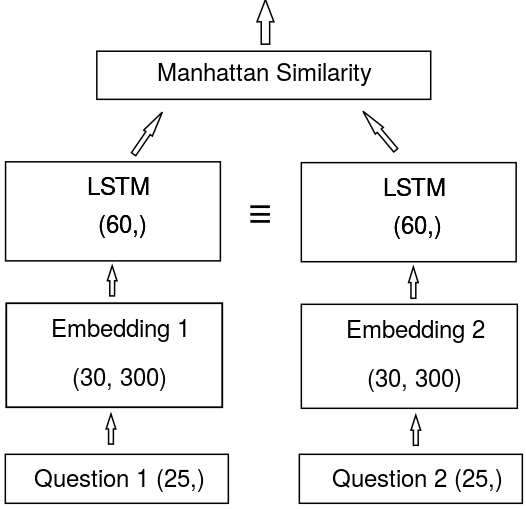
\includegraphics[scale=.2]{MaLSTM}
		\centering
      }}
      %\includegraphics[scale=1.0]{figurefile}
      \caption{Manhattan Siamese LSTM archetecture, annotated with output dimension at each layer. Weights of each LSTM layer are tied (Siamese).}
      \label{figurelabel}
   \end{figure}



\section*{STATEMENT OF CONTRIBUTION}

The preferred spelling of the word ÒacknowledgmentÓ in America is without an ÒeÓ after the ÒgÓ. Avoid the stilted expression, ÒOne of us (R. B. G.) thanks . . .Ó  Instead, try ÒR. B. G. thanksÓ. Put sponsor acknowledgments in the unnumbered footnote on the first page.



%%%%%%%%%%%%%%%%%%%%%%%%%%%%%%%%%%%%%%%%%%%%%%%%%%%%%%%%%%%%%%%%%%%%%%%%%%%%%%%%

References are important to the reader; therefore, each citation must be complete and correct. If at all possible, references should be commonly available publications.



\begin{thebibliography}{99}

\bibitem{c1} Daniel Jurafsky and James H. Martin. 2009. Speech and Language Processing (2nd Edition). Prentice-Hall, Inc., Upper Saddle River, NJ, USA.
\bibitem{c2} Daniel Jurafsky and James H. Martin. 2017 Speech and Language Processing. (3rd Edition Draft) 
\bibitem{c3} Lin, C., and Hovy, E. 2003. Automatic evaluation of summaries
using n-gram co-occurrence statistics. In Proceedings of Human
Language Technology Conference .
\bibitem{c4} Xin Li, Dan Roth, Learning Question Classifiers. COLING'02, Aug., 2002.
\bibitem{c5} Rajaraman, A.; Ullman, J.D. (2011). "Data Mining". Mining of Massive Datasets. pp. 1–17.
\bibitem{c6} Rada Mihalcea, Courtney Corley, and Carlo Strapparava. Corpus-based and knowledge-based measures of text semantic similarity. In AAAI’06, July 2006.
\bibitem{c7} George A. Miller (1995). WordNet: A Lexical Database for English. 
Communications of the ACM Vol. 38, No. 11: 39-41.
\bibitem{c8} Jonas Mueller and Aditya Thyagarajan. Siamese Recurrent Architectures for Learning Sentence Similarity. In AAAI, 2016
\bibitem{c9} Rocktäschel, Grefenstette, Hermann, Kočiský and Blunsom. Reasoning about Entailment with Neural Attention. in: International Conference on Learning Representations (ICLR). 2016
\bibitem{c10} A. Joulin, E. Grave, P. Bojanowski, T. Mikolov, Bag of Tricks for Efficient Text Classification
\bibitem{c11} Scikit-learn: Machine Learning in Python, Pedregosa et al., JMLR 12, pp. 2825-2830, 2011.


\end{thebibliography}




\end{document}
